% 原印刷225--232页／PDF物理249--256；§6.2，止于§6.3之前.
\subsection{Angenent--Hacker--Tannenbaum方法}\label{sec:6.2}
本节的算法源于\cite{b19}提出并研究的一个有趣的极小化流（另见\cite{b191}）. 主要想法是从给定密度$f$与目标测度$\nu$之间的一个可行传输映射$\mathrm T$出发（假设$f$在性质良好的紧区域$\Omega$上光滑且严格为正；目前不对$\nu$作任何正则性要求），然后通过与向量场$\mathbf v$的流复合，缓慢地随时间重新排列$\mathrm T$的值，即考虑$\mathrm T\circ(Y_t)^{-1}$而不是$\mathrm T(x)$；其中，如常，$Y_t(x):=y_x(t)$是
\[
\begin{cases}
y_x'(t)=\mathbf v_t(y_x(t)),\\
y_x(0)=x
\end{cases}
\]
的解.

\begin{figure}[htbp]
\centering
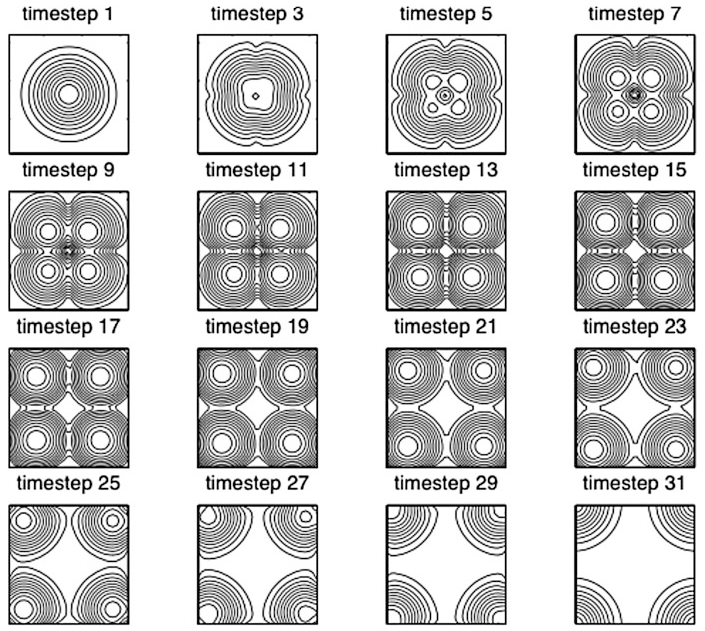
\includegraphics[width=.98\linewidth]{assets/ch06-fig-6-1.pdf}
\caption{二维环面上的一个高斯分布与将其平移向量$(1/2,1/2)$所得的同一高斯分布之间的测地线. 注意，为避开割迹（见\autoref{sec:1.3.2}），初始密度分裂为四部分. 图片经许可取自\cite{b34}.}\label{fig:6.1}
\end{figure}

选择向量场$\mathbf v_t$时，既要使由$Y_t(x):=y_x(t)$定义的映射$Y_t$保持测度$f$，又要降低Monge成本
\[
M(\mathrm T)=\int c(x,\mathrm T(x))f(x)\,\mathrm dx
\]
的值. 假设成本$c$光滑（例如$C^1$；后面将考察二次成本这一特殊情形）.

首先要计算成本函数的导数：令$\mathrm T_t(x):=\mathrm T(y_x(-t))$，其中$y$定义为自治向量场$\mathbf v$的流. $\mathbf v$保持测度$f$的条件，是
\[
\partial_t\varrho_t+\nabla\cdot(\varrho_t\mathbf v)=0
\qquad\text{且 }\varrho_0=f
\]
的解为关于时间不变的密度$\varrho_t=f$. 这要求$\nabla\cdot(f\mathbf v)=0$. 为简便，令$\mathbf w=f\mathbf v$. 选择满足此条件的$\mathbf v$，便可以写出
\[
\begin{aligned}
\frac{\mathrm d}{\mathrm dt}
\left(\int_\Omega c(x,\mathrm T(y_x(-t)))f(x)\,\mathrm dx\right)
&=\frac{\mathrm d}{\mathrm dt}
\left(\int_\Omega c(y_x(t),\mathrm T(x))f(x)\,\mathrm dx\right)\\
&=\int_\Omega\nabla_xc(y_x(t),\mathrm T(x))\cdot y_x'(t)f(x)\,\mathrm dx\\
&=\int_\Omega\nabla_xc(y_x(t),\mathrm T(x))
\cdot\mathbf v(y_x(t))f(x)\,\mathrm dx,
\end{aligned}
\]
在$t=0$时，导数等于$\int_\Omega\nabla_xc(x,\mathrm T(x))\cdot\mathbf v(x)f(x)\,\mathrm dx$. 上面的计算利用了$Y_{-t}$保持测度$f$以及它的逆为$Y_t$这一事实（对与时间无关的向量场$\mathbf v$，这确实成立）.

这里重新得到了最优传输理论的重要一部分：若$\mathrm T$最优，则向量场$\nabla_xc(x,\mathrm T(x))$必与所有无散向量场$\mathbf w$正交，因而它是梯度（见\autoref{obj:1.15}）. 特别在$c(x,y)=\frac12|x-y|^2$时，这给出$x-\mathrm T(x)=\nabla\varphi(x)$，从而$\mathrm T$本身也是梯度. $\mathrm T$是凸函数而非任意函数的梯度这一事实，来自二阶最优性条件，至少在正则性充分时如此（见\autoref{ex:44}）.

然而，这里的目标并非研究最优$\mathrm T$的结构，而是从非最优的$\mathrm T$出发并改进它. 为此，必须选择合适的向量场$\mathbf v$. 我们将通过产生一个流$\mathrm T_t$来实现这一点，并在每个时刻$t$以某种巧妙方式选择向量场$\mathbf v$. 因而它将不再是自治的. $\mathbf v$有多种可能的选择，但先从最简单的出发：我们看到，成本$M$的导数由$\int_\Omega\xi\cdot\mathbf w$给出，其中$\xi(x)=\nabla_xc(x,\mathrm T(x))$，$\mathbf w=f\mathbf v$. 由于$\int_\Omega\xi\cdot\mathbf w$是$L^2$中的内积，这便识别出了$M$关于$L^2$结构的梯度，这里限制在保持测度的无穷小位移的集合上（即加上约束$\nabla\cdot\mathbf w=0$）. 若希望$\|\mathbf w\|_{L^2}$有界，最优的$\mathbf w$选择，是取$-\xi$到无散向量场所成向量空间上的投影. 关于这一散度约束所配的边界条件，如常选择Neumann条件$\mathbf w\cdot\mathbf n=0$；为保持测度而不使质量流出$\Omega$，也正需要这些条件.

\begin{sourcebox}{备忘：Helmholtz分解}\label{box:6.2}\index{H076@Helmholtz分解（Helmholtz decomposition）|hyperpage}
给定向量场$\xi\in L^2(\Omega;\mathbb R^d)$，总可以将其写成梯度与无散向量场之和：$\xi=\nabla u+\mathbf w$，其中$u\in H^1(\Omega)$，$\nabla\cdot\mathbf w=0$（分布意义下）. 若要求$u\in H_0^1(\Omega)$或$\mathbf w\cdot\mathbf n=0$，则分解唯一；后一个条件取弱意义，即与零散度条件一起，表示对一切$\phi\in C^1(\Omega)$都有$\int\mathbf w\cdot\nabla\phi=0$.

这些分解具有变分起源：实际上，求解
\[
\min\left\{\int|\xi-\nabla u|^2:u\in H_0^1(\Omega)\right\}
\]
可得第一种分解，而求解
\[
\min\left\{\int|\xi-\nabla u|^2:u\in H^1(\Omega),\quad\int u=0\right\}
\]
可得第二种分解（若$\Omega$连通）. 两种情形中，$\mathbf w$的零散度条件都来自关于$u$的最优性条件.

注意，$\nabla u$是$\xi$到$L^2$梯度集合上的投影（第一种情形为$H_0^1$函数的梯度），因而$\mathbf w$是到无散向量场集合上的投影（第二种情形还带Neumann条件）.

投影$\mathbf w=P[\xi]$可以通过$\nabla\cdot\xi=\nabla\cdot\mathbf w+\Delta u$来计算，即$\mathbf w=\xi-\nabla(\Delta^{-1}(\nabla\cdot\xi))$.
\end{sourcebox}

因此，我们寻找一族传输映射$\mathrm T_t$、一个流$Y_t$和一个向量场$\mathbf w_t$，满足以下条件：
\begin{itemize}
\item 在每个时刻$t$，$\mathrm T_t$定义为$\mathrm T_t=\mathrm T\circ(Y_t)^{-1}$；
\item 映射$Y_t$是时变向量场$\mathbf v_t$的流，$\mathbf v_t$通过$f\mathbf v_t=\mathbf w_t$定义；
\item 向量场$\mathbf w_t=P[-\xi_t]$，其中$P$是到满足$\mathbf w\cdot\mathbf n=0$的无散向量场上的投影，$\xi_t=\nabla_xc(x,\mathrm T_t(x))$.
\end{itemize}
可以写出$\mathrm T_t$满足的偏微分方程，即传输方程$\partial_t\mathrm T_t+\mathbf v_t\cdot\nabla\mathrm T_t=0$.

\begin{sourcebox}{备忘：线性传输方程}\label{box:6.3}\index{T152@传输方程（transport equation）|hyperpage}
给定光滑向量场$\mathbf v_t$、它的流$Y_t(x)=y_x(t)$（如常，$y_x'(t)=\mathbf v_t(y_x(t))$且$y_x(0)=x$）以及光滑函数$g$，定义$g_t=g\circ Y_t^{-1}$. 则有
\[
\partial_tg_t+\mathbf v_t\cdot\nabla g_t=0.
\]
事实上，可以写成$g_t(y_x(t))=g(x)$，再对时间求导，就得到上式. 只要$\mathbf v_t$保持Lipschitz连续，它的弱形式就对任意$g\in L^1$有效：可以取光滑逼近函数序列$g_n\to g$，写出$\iint g_n\circ Y_t^{-1}(\partial_t\varphi+\mathbf v_t\cdot\nabla\varphi)$，作换元$y=Y_t^{-1}(x)$，然后取极限.

这个方程称为传输方程. 它与连续性方程相似，但不是守恒形式，$g$的质量不随时间守恒. 相反，$g$的$L^\infty$界得到保持，因为$g_t$的值与$g=g_0$的值相同. 传输方程与连续性方程在某种意义上互为对偶：若固定向量场$\mathbf v$，并取$\partial_t\varrho_t+\nabla\cdot(\varrho_t\mathbf v_t)=0$的光滑解$\varrho_t$及$\partial_tg_t+\mathbf v_t\cdot\nabla g_t=0$的光滑解$g_t$，则有
\[
\begin{aligned}
\frac{\mathrm d}{\mathrm dt}\left(\int g_t\,\mathrm d\varrho_t\right)
&=\int(\partial_tg_t)\varrho_t+\int g_t(\partial_t\varrho_t)\\
&=-\int\varrho_t\mathbf v_t\cdot\nabla g_t
-\int g_t\nabla\cdot(\varrho_t\mathbf v_t)=0.
\end{aligned}
\]
\end{sourcebox}

现在，在上述选择下形式地计算$M(\mathrm T_t)$关于时间的导数：
\[
\begin{aligned}
\frac{\mathrm d}{\mathrm dt}M(\mathrm T_t)
&=\frac{\mathrm d}{\mathrm dt}\left(\int c(x,\mathrm T_t)f\right)
=\int\nabla_yc(x,\mathrm T_t)(\partial_t\mathrm T_t)f\\
&=-\int\nabla_yc(x,\mathrm T_t)\cdot\nabla\mathrm T_t\cdot\mathbf w_t.
\end{aligned}
\]
继续使用$\nabla[c(x,\mathrm T_t(x))]=\nabla_xc(x,\mathrm T_t(x))+\nabla_yc(x,\mathrm T_t(x))\nabla\mathrm T_t(x)$，以及来自$\nabla\cdot\mathbf w_t=0$的$\int\nabla[c(x,\mathrm T_t(x))]\cdot\mathbf w_t(x)\,\mathrm dx=0$. 因而得到
\[
\begin{aligned}
\frac{\mathrm d}{\mathrm dt}M(\mathrm T_t)
&=\int\nabla_xc(x,\mathrm T_t)\cdot\mathbf w_t(x)
=\int\xi_t\cdot\mathbf w_t\\
&=-\int\xi_tP[\xi_t]=-\|P[\xi_t]\|^2\le0.
\end{aligned}
\]
这表明所提出的流使$M(\mathrm T_t)$随时间下降，且$M(\mathrm T_t)$的值平稳，当且仅当$P[\xi_t]=0$，即$\xi_t$是梯度.

\cite{b19}证明了上述流的局部存在性，即
\[
\begin{cases}
\partial_t\mathrm T_t+\mathbf v_t\cdot\nabla\mathrm T_t=0,\\
\nabla\cdot(f\mathbf v_t)=0,\quad\mathbf v_t\cdot\mathbf n=0,\\
-\nabla_xc(x,\mathrm T_t)=f\mathbf v_t+\nabla u_t,\\
\mathrm T_0\text{ 给定}.
\end{cases}
\]
（第二、三行可以替换为$\mathbf v_t=\xi_t-\nabla(\Delta^{-1}(\nabla\cdot\xi_t))$，其中$\xi_t=\nabla_xc(x,\mathrm T_t)$；这避免引入新变量$u_t$，但在方程中引入了非局部项.）还证明了，当$t\to\infty$时，$\mathrm T_t$的极限只能是$\mathrm T_0$的那些满足$\nabla_xc(x,\mathrm T)$为梯度的重排$\mathrm T$. 论文也研究了以传输方案代替传输映射的更一般情形，不过为简便起见，我们不介绍这一深入情形. 但应注意，\phantomsection\label{idx:i153-p229}\index{T153@扭曲条件（twist condition）|hyperpage}
对于不满足扭曲条件的成本$c$，传输方案的框架不可避免. 事实上，一般不可能在$t\to\infty$时收敛到最优传输映射，只因为这样的映射可能不存在.

同一篇论文\cite{b19}还提出了向量场$\mathbf v$的其他选择，特别是“正则化”的流（即对上述$\mathbf w_t$施加正则化核；在此情形证明了全局存在性）. 还可以对流作局部选择：用坐标写，可以取$w^j=\xi^i_{ji}-\xi^j_{ii}$（上标表示分量，下标表示求导）. 可以验证，这一选择同样保证$M(\mathrm T_t)$随时间下降.

虽然如前所述这一方法对任意成本都具有一般性，但它主要用于二次成本情形. 此时的想法可以粗略概括为：“从一个可行传输映射出发，然后把它梯度化”（即缓慢地将其变成梯度）.

对$\xi_t=x-\mathrm T_t$，方程变成
\[
\begin{cases}
\partial_t\xi_t-\mathbf v_t+\mathbf v_t\cdot\nabla\xi_t=0,\\
\mathbf v_t=\dfrac1f\left(\xi_t-\nabla(\Delta^{-1}(\nabla\cdot\xi_t))\right),\\
\xi_0(x)=x-\mathrm T_0(x)\text{ 给定}.
\end{cases}
\]
从实现角度看（见\cite{b20}），上面的系统已被离散并求解，其中传输方程使用迎风格式（粗略说，就是根据输运向量场$\mathbf v$各分量的符号，选择左侧或右侧中心导数的有限差分法），Laplacian的求解使用标准求解器（如Matlab的Poisson求解器）. 每次时间迭代的复杂度为$N\log N$量级，其中$N$是空间离散化的像素数.

AHT流已用于数值计算，它既有优点也有缺点. 虽然它主要用于二次情形，但也可用于许多光滑成本，因此是很一般的方法. 不过，从数值角度看，实现存在一些困难，而且还有要求密度严格为正的缺点. 此外，它收敛到最优映射这一点完全没有得到证明. 在二次情形下，这一问题很容易理解. 注意，这里并不是说严格的收敛结果：问题在于，这个流旨在收敛到成本$M$的临界点，这对二次情形意味着传输$\mathrm T$是梯度映射. 但没有任何东西保证它是凸映射的梯度！

先验地，甚至可能得到凹函数的梯度（即二次成本下最坏的映射，见\autoref{ex:2}）. 由于该流在尚未遇到临界点时具有$M(\mathrm T_t)$随时间严格下降的性质，这一情形容易排除（唯一可能是从凹函数梯度$\mathrm T_0$出发，而这很容易避免）. 但极限仍可能是其他任意梯度.

\cite{b86}讨论了这些问题. 根据\cite{b19,b20}，为改善结果、提高收敛到正确传输映射的可能性，一个好办法是选择良好的初始猜测$\mathrm T_0$. 文献提出了几种专用于二次情形的选择（\phantomsection\label{idx:i37-p230}\index{D037@Dacorogna--Moser方法（Dacorogna-Moser）|hyperpage}
包括Dacorogna--Moser传输映射，见\autoref{sec:4.2.3}中的\autoref{box:4.3}），\phantomsection\label{idx:i86-p230}\index{K086@Knothe映射（Knothe map）|hyperpage}
但至少乍看起来，最合适的是Knothe传输（见\autoref{sec:2.3}）. 事实上，作此选择，初始传输映射的Jacobi矩阵为三角形，且特征值为正. 除了先前假设，再假设$\nu$绝对连续，其密度$g(x)$有正常数的上下界. 已知映射$\mathrm T_t$对每个$t$都满足$(\mathrm T_t)_\#f=g$，故$|\det(D\mathrm T_t)|$的值永不为零（下界为$\inf f/\sup g$）. 若一切光滑，就意味着行列式的符号保持不变，而且任何特征值都不可能为零（\cite{b86}也强调了这一点）. 不幸的是，$D\mathrm T_t$的特征值在$t=0$时为实数（若选择Knothe映射），在$t=\infty$时也为实数（由于是梯度，Jacobi矩阵对称），但演化过程中没有任何东西阻止特征值变成复数，从$]0,+\infty[$到$]-\infty,0[$而不经过零！（尽管这似乎不大可能发生，因为$\mathbf v$的选择恰好迫使$\mathrm T_t$越来越接近梯度集合，而梯度并不喜欢复特征值.）

如果一切光滑，有一种不存在歧义的简单情形，就是二维情形. 可以给出一个直接的命题.

\begin{proposition}\label{obj:6.3}
设$(\xi_t,\mathbf v_t)$是二次情形下AHT系统的一个光滑解，$\mathrm T_t(x)=x-\xi_t(x)$是给定的两个光滑密度$f,g\in\mathscr P(\Omega)$之间的传输映射，其中$\Omega\subset\mathbb R^2$是二维光滑凸有界区域. 假设对每个$x$都有$\det(D\mathrm T_0(x))>0$. 再假设当$t\to\infty$时$\mathrm T_t\to\mathrm T_\infty$于$C^1(\Omega)$，且演化非平凡（即存在$t$使$\mathrm T_t\ne\mathrm T_0$）. 那么$\mathrm T_\infty$是凸函数的梯度，因而最优.
\end{proposition}
\begin{proof}
由上面的考虑，
\begin{equation}\label{eq:6.1}
M(\mathrm T_0)-M(\mathrm T_t)=\int_0^t\|P[\xi_t]\|_{L^2}^2\,\mathrm dt.
\end{equation}
这蕴含$\int_0^\infty\|P[\xi_t]\|_{L^2}^2\,\mathrm dt<\infty$，并且至少沿某个序列$t_n\to\infty$有$P[\xi_{t_n}]\to0$于$L^2(\Omega)$. 从而$P[\xi_\infty]=0$，因为$\xi_{t_n}\to\xi_\infty:=x-\mathrm T_\infty(x)$于$C^1$；于是$\xi_\infty$和$\mathrm T_\infty$都是梯度. 需要证明$\mathrm T_\infty$是凸函数的梯度，即如今对称的矩阵$D\mathrm T_\infty$的两个特征值都为正（记住我们在$\mathbb R^2$中）.

已知$t\mapsto\det(D\mathrm T_t(x))$关于时间连续，在$t=0$时为正，且不可能为零. 由$C^1$收敛性，对每个$x$都有$\det(D\mathrm T_\infty(x))>0$. 因此，$D\mathrm T_\infty(x)$的特征值同号（对每个固定的$x$）.

现在看$\operatorname{Tr}(D\mathrm T_\infty(x))$. 这是$x$的连续函数，且不可能为零. 事实上，若它在某处为零，则该点的两个特征值就会异号. 因此，这个迹的符号关于$x$恒定. 注意，这只在$t=\infty$时成立，因为对$t\in]0,\infty[$，先验地可能有复特征值.

若排除$\operatorname{Tr}(D\mathrm T_\infty(x))$处处小于零的情形，证明就完成了. 但这一情形对应于$\mathrm T_\infty$是凹函数的梯度（再次回忆，在二维中，行列式为正且迹为负，蕴含二维负定）. 而凹函数对应二次情形下最坏的传输（见\autoref{ex:2}）. 这是不可能的，因为由\eqref{eq:6.1}有$M(\mathrm T_\infty)<M(\mathrm T_0)$（除非曲线$t\mapsto\mathrm T_t$恒定）.
\end{proof}

注意，Knothe传输与Dacorogna--Moser传输映射都满足上述定理关于初始条件的假设.

不幸的是，上述证明确实是二维的，因为我们把正的对称矩阵刻画为迹与行列式都为正的矩阵. 此外，在实践中几乎不可能保证上述定理的假设，只能经验性地观察到收敛.

\begin{openproblem}[AHT的收敛]
即使假设光滑性及很强的收敛性，证明在高于二维的维数中，从Knothe和／或Dacorogna--Moser映射初始化的AHT流收敛到最优映射；并在二维中，以尽可能弱的假设证明严格结果.
\end{openproblem}
